\section{Basic Concept}

\underline{Amdahl's law} \parencite{book6}:

\begin{figure}[h!]\centering
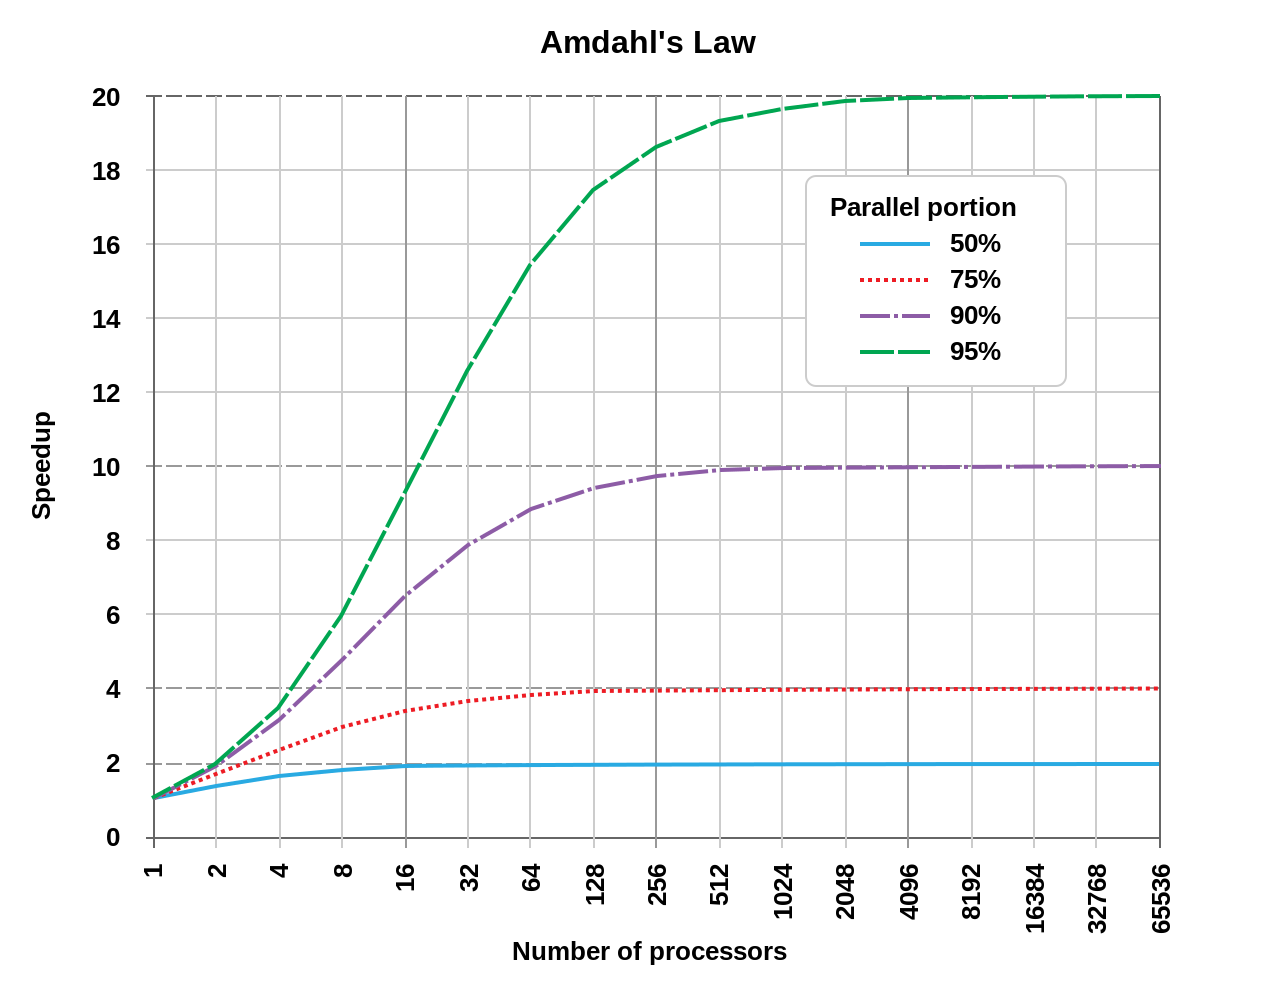
\includegraphics[scale=0.8]{amdahls-law.png}
\caption{
...
}
\label{fig:admLaw}
\end{figure}

\begin{itemize}
\item “the contention that the organization of a single computer has reached its limits and that
truly significant advances can be made only by interconnection of a multiplicity of computers” \parencite[see][p80]{inbook1}; can be transferd on single and multi-core processors or even on multithreading, but in fact, like Amdahl claimed too, adressing hardware, and nowerdays switching context time was not considered here!
Valiant noted in 1990, “no substantial impediments to general-purpose parallel
computation” exist \parencite[see][p85]{inbook1}, though there are limits, as shown \parencite[seein Sec. 10][p85]{inbook1}.

\newpage

\item “the fraction of the computational load... associated with data management housekeeping ... accounts for 40\% of the executed instructions”, "this overhead appears to be sequential so that it is unlikely to be amenable to parallel processing techniques” \parencite[see][p80]{inbook1}; amount of overhead (data management and adressing based on hardware restricitons), which can not be parallelized and reduces the factor of speed increase after parallelization. According to Amdahl, this factor can be reduced, but not with "parallel processing techniques", probably with more precisely and efficent hardware.
\item a resisting "upper limit on speedup [exists] and therefore, apart from the sequential fraction (the so called non parallelizabled overhead), the remaining computations are perfectly parallelizable" \parencite[see][p81]{inbook1}
\item the law in general: Let t\textsubscript{1} be the time taken by one processor solving a computational problem and t\textsubscript{p} be the time taken by p processors solving the same problem. Finally let us denote the supposed inherently sequential fraction of instructions by f. Then, according to Amdahl, t\textsubscript{p} = t\textsubscript{1} (f+(1-f)/p) and the speedup obtainable by p processors can be expressed as:

	
\[ \frac{t_1}{t_p} = \frac{1}{f + (1 - f) / p)} \]
\end{itemize}

\newpage

\subsection{Principles of Parallel Computing}

\textbf{Emphasises design}:
Amdahl's law highlights the pitfalls of looking for
sticking-plaster speed-ups in serial programs –
design for concurrency \parencite[see][p4]{article6}
\\\\\textbf{Aim of concurrency and their effects} on program structure or implementation \parencite[see][p5]{article6}:
\begin{itemize}
  \item \underline{Flexibility}: Environments will be more heterogeneous.
  \item \underline{Efficiency}:	parallel for a speed-up purposes, more pitfalls (memory latency, thread overheads etc.)
  \item \underline{Simplicity}:	Parallel codes will be more complicated. All the more reason to strive for maintainable, understandable programs.
\end{itemize}

\newpage

\section{Definition of parallel mathematical computations}


...\newpage

\section{Parallel Computer Architecture}

...\parencite[see][p9]{book1} \\
...examples of parallelism \parencite[see][p11]{book1}

\subsection{Flynn's Taxonomy of Parallel Architectures}

...\parencite[see][p5]{internet1}\\
...\parencite[see][p13]{book1}\\
...\parencite[see][p4]{book5}\\
...\parencite[see][p2]{book6}\\

\subsection{Thread Level Parallism}

...\parencite[see][p24]{book1}

\section{Parallel Programming Models}

\textbf{Steps to evaluate a proper parallel design} \parencite[see][p6]{article6}:
\begin{enumerate}
	\item Finding Concurrency
	\item Algorithm Structure
	\item Supporting Structures
	\item Implementation Mechanisms
\end{enumerate}

\newpage

\subsection{Classification of Parallel Programming Models}

\subsubsection{Process Interaction}

...\parencite[see][p4]{internet1}

\subsubsection{Problem decomposition}

...\parencite[see][p105 ff.]{book1}